\documentclass[10pt,twocolumn,letterpaper]{article}

% \usepackage{cvpr}
\usepackage{times}
\usepackage{epsfig}
\usepackage{graphicx}
\usepackage{amsmath}
\usepackage{amssymb}
\usepackage{makecell}

% Include other packages here, before hyperref.

% If you comment hyperref and then uncomment it, you should delete
% egpaper.aux before re-running latex.  (Or just hit 'q' on the first latex
% run, let it finish, and you should be clear).
\usepackage[breaklinks=true,bookmarks=false]{hyperref}


\begin{document}


%%%%%%%%% TITLE
\title{Learn transferable features for semantic image segmentation in the presence of label noise}

\author{First Author\\
Institution1\\
Institution1 address\\
{\tt\small firstauthor@i1.org}
% For a paper whose authors are all at the same institution,
% omit the following lines up until the closing ``}''.
% Additional authors and addresses can be added with ``\and'',
% just like the second author.
% To save space, use either the email address or home page, not both
\and
Second Author\\
Institution2\\
First line of institution2 address\\
{\tt\small secondauthor@i2.org}
}

\maketitle
%\thispagestyle{empty}


%%%%%%%%% ABSTRACT
\begin{abstract}
   The ABSTRACT HERE
\end{abstract}

%%%%%%%%% BODY TEXT
\section{Bullet points}


\paragraph{Data for Semantic Segmatation}
\begin{itemize}
  \item Rich unlabeled data, but lack of annotations
  \item (Conventially) The annotations need to be:
  \begin{itemize}
    \item \textbf{precise}: no false positive
    \item \textbf{complete}: no false negative
    \item \textbf{consistent}: no misclassification
  \end{itemize}
  \item ``Lazy annotating'': Annotations that
  \begin{itemize}
      \item contain imprecise annotations
      \item are imcomplete
      \item contain misclassification
  \end{itemize}
  \item Motivation:
  \begin{itemize}
    \item Correcting annotation errors take much more effort than annotating more data
    \item Annotating errors can be compensated with appropriate assumptions
  \end{itemize}
\end{itemize}


\paragraph{Methods}
\begin{itemize}
  \item Incomplete annotations: Positive and Unlabelled learning
  \item Imprecise annotations: Learning ``objectiveness''
\end{itemize}


\section{Introduction}
\label{introduction}

%%%%%%%%%%%%%%%%%%%%%%%%%%%%%%%%%%%%%%%%%%%%%%%%%%%%%%%%%%%%%%%%%%%%%%
%%%%%%%% TEXT Why transfer learning?
%%%%%%%%%%%%%%%%%%%%%%%%%%%%%%%%%%%%%%%%%%%%%%%%%%%%%%%%%%%%%%%%%%%%%%

% \noindent \textit{Why transfer learning? \\
% Segmentation model benefits from transfer learning.
% \begin{itemize}
%   \item Success of CNN benefits from large-scale data whereas segmentation datasets are small
%   \item Collecting segmentation in one domain on a large scale can be difficult.
%   \item One can transfer pre-trained CNN model to train with limited training samples access.
% \end{itemize}
% }

The state-or-the-art convolution neural nets benefits from transferring weights from convolutional neural network (CNN) models trained with a subset of images from ImageNet, referred to as the \textit{ImageNet models}.\cite{long2015fully,chen2016deeplab,he2017mask}
These ImageNet CNN models\cite{krizhevsky2012imagenet,simonyan2014very,szegedy2015going,he2016deep} trained for object recognition task benefit from the availability of a large-scale supervised dataset, the ILSRVC dataset\cite{russakovsky2015imagenet} which contains around 1.2 million labeled images.
In contrast to object recognition tasks, it is difficult to collect a dataset for semantic segmentaiton on that large scale.
This difficulty is natural because it costs much more efforts for people to segment than to classify an image.
Therefore, scales of semantic segmentation datasets are normally much smaller than object recognition dataset.
For instance, one of the largest segmentation datasets, Microsoft COCO2014\cite{lin2014microsoft}, contains 123,287 images for 80 object categories, smaller than the ILSRVC dataset by a factor of 10 approximately.
% the Pascal VOC2012 challenge\cite{everingham2015pascal} provides a segmentation dataset with only 9,993 segmented images for 20 object categories;
% The PASCAL-context Dataset\cite{mottaghi2014role} enriches the PASCAL VOC dataset by segmenting all 11,530 training images for 540 categories;
Therefore, semantic segmentation models are often trained with constraints of limited numbers of available training images.
A commonly used method for improving segmentation performance in the limitation of lacking training samples is to transfer weights from the pre-trained ImageNet models.\cite{long2015fully,chen2016deeplab}


%%%%%%%%%%%%%%%%%%%%%%%%%%%%%%%%%%%%%%%%%%%%%%%%%%%%%%%%%%%%%%%%%%%%%%
%%%%%%%% TEXT Why pre-training with segmentation?
%%%%%%%%%%%%%%%%%%%%%%%%%%%%%%%%%%%%%%%%%%%%%%%%%%%%%%%%%%%%%%%%%%%%%%

% \noindent \textit{Why pre-training with segmentation? \\
% ImageNet models have limitations.
% \begin{itemize}
%   \item Disimilarity in domain of interest for training images
%   \item Architecture limitation of ImageNet models. (3D ConvNet)
% \end{itemize}
% }

However, there can be limitations for these ImageNet models to significantly improve performance for a segmentation model.
Firstly, the ImageNet models were trained with relatively low resolution natural images.
In some domains of interest, training images can be non-natural, for example, aerial images, images from bird's eye view, and medical images;
In other domains, mages may have different lighting conditions from the ImageNet images such as photos taken in a dark warehouses;
Images to be segmented may also have higher resolution than the ImageNet ones.
To train a segmentation model in these domains, it can be beneficial to fine-tune the ImageNet model using a similar dataset in the domain of interest if there exists one.
Secondly, the ImageNet models cannot be applied directly to RGB-D images or 3D images like CT scans and MRI scans in 3D.
Lastly, segmentation models may have different design thinkings from classification models due to the inherent differences of the two tasks.
For example, features' translation invariance and reduced resolution for object recognition CNN models can reduce localization accuracy for segmentation.\cite{zheng2015conditional,chen2016deeplab}
The challenges in adapting ImageNet models for segmentation tasks can result in different architectures for segmentation models\cite{zheng2015conditional}.
% Even adapted segmentation models\cite{long2015fully,chen2016deeplab,he2017mask} have components not from the original ImageNet models.
Therefore, a model pre-trained with segmentation datasets in a similar domain can be useful to achieve good segmentation performance with a small training set.

% \footnote{The KITTI Vision Benchmark Suite http://www.cvlibs.net/datasets/kitti/}

%%%%%%%% ? Deeplab https://arxiv.org/pdf/1606.00915.pdf
%%%%%%%% In particular we consider three challenges in the application of DCNNs to semantic image segmentation: (1) reduced feature resolution, (2) existence of objects at multiple scales, and (3) reduced localization accuracy due to DCNN invariance.
%%%%%%%% ? CRFasRNN http://www.robots.ox.ac.uk/~szheng/papers/CRFasRNN.pdf
%%%%%%%% Firstly, traditionalCNNs have convolutional filters with large receptivefields and hence produce coarse outputs when restructured to produce pixel-level labels [37]
%%%%%%%% Secondly, CNNs lack smoothness constraints that encourage label agreement between similar pixels, and spatial and appearance consistency of the labelling output


%%%%%%%%%%%%%%%%%%%%%%%%%%%%%%%%%%%%%%%%%%%%%%%%%%%%%%%%%%%%%%%%%%%%%%
%%%%%%%% TEXT Why labels are noisy?
%%%%%%%%%%%%%%%%%%%%%%%%%%%%%%%%%%%%%%%%%%%%%%%%%%%%%%%%%%%%%%%%%%%%%%

% \noindent
% \textit{Why labels are noisy?
% \begin{itemize}
%   \item Crowd-sourcing data is noisy by nature.
%   \item ``gold standard'' itself can be ambiguous.
%   \item There exists free available noisy segmentation datasets
% \end{itemize}
% }

The pre-training segmentation datasets may, however, contain label noises, and the existence of segmentaion noises should not magnificently affect the transferability of pre-trained weights.
The use of crowd-sourcing platform like Mechanical Turk is common nowadays to collect datasets on a large scale.
However, it is natural for crowd-sourcing workers to make mistakes as a result of lack of expertise, inherent ambiguity of tasks or unconscious bias.
Enormous efforts are required, according to \cite{lin2014microsoft,everingham2015pascal}, to ensure the correctness of segmentations.
A slight decrease in percentage of segmentation errors, such as from 1\% to 0\%, may require extraordinary extra efforts due to the difficulty of identifying errors.
If not requiring ``gold standard'' segmentations, the efforts saved for correctness can be made for segmenting more images so that the result segmentations can be larger in numbers though traded with the existence of label noises.
% Trade-offs need to be made between the impact of by label noise and the gain of a larger dataset.
In some domains, for example medical imaging, the ``gold standard'' itself can be ambiguous and cause disagreements among experts.
\footnote{M: But that's OK or not?  This is what probabilities solve...}
Besides, freely available labels may exist for particular tasks, as alternatives to manual annotations.
But these labels often contain structural noises depending on the way they were created.
For example, one can use digital maps, like OpenStreetMap, to segment aerial images.
These segmentations constructed from maps would suffer from the incomplete annotation as well as registration problems.\cite{mnih2012learning}
% Besides, Pl@ntNet\footnote{https://identify.plantnet-project.org/}, a crowdsourcing platform, provide millions of images of plants and corresponding labels which may or may not be correct.
Ideally, the use of these noisy datasets for pre-training should not affect the result weights transferring to another dataset.
If negative influences of label noises on weights transferability were remarkable, methods of compensating the noises then become relevant.


%%%%%%%%%%%%%%%%%%%%%%%%%%%%%%%%%%%%%%%%%%%%%%%%%%%%%%%%%%%%%%%%%%%%%%
%%%%%%%% TEXT What types of noises exist and motivate them?
%%%%%%%%%%%%%%%%%%%%%%%%%%%%%%%%%%%%%%%%%%%%%%%%%%%%%%%%%%%%%%%%%%%%%%

% \noindent \textit{What types of noises exist and motivate them?
% \begin{itemize}
%   \item Inexaustive segmentation
%   \item Misclassification
%   \item False segmentations
% \end{itemize}
% }

\paragraph{Segmentation noises}
Noises of different kinds can exist in segmentation labels, for example, inexaustive segmentation, misclassification of segments, false segmentating, over-segmenting, under-segmenting, etc.
In particular, we consider only noises happen to labels for the whole segments instead of individual pixels, assuming the outline of segments are always correct.
That leaves us three types of noises: inexaustive segmentation, misclassification and false segmentation.
Inexaustive segmention, i.e., there exists objects left unsegmented, is one of the most frequent noises.
A typical situation of inexaustive segmentation is when images contain huge amounts of objects of the same kind, e.g. a flock of sheeps or a pile of products.
Misclassfication of segments can be avoided to some extent by asking annotators to segment one category at a time.\cite{lin2014microsoft}
Occasional misclassified objects may nevertheless still exist because of the ambiguity of category definations, for example, the misclassified bears and teddy bears in the Microsoft COCO dataset.
False segmentation denotes objects not of interest wrongly segmented as objects of interest.
It may occur due to unclear category defination, the lack of knowledge or simply visual bias.
We synthesized these three types of noises with a well-annotated dataset and studied their influences to the trained weights transferability separately.


%%%%%%%%%%%%%%%%%%%%%%%%%%%%%%%%%%%%%%%%%%%%%%%%%%%%%%%%%%%%%%%%%%%%%%
%%%%%%%% TEXT Why binarizing classes?
%%%%%%%%%%%%%%%%%%%%%%%%%%%%%%%%%%%%%%%%%%%%%%%%%%%%%%%%%%%%%%%%%%%%%%

% \noindent \textit{Why binarizing classes?}

{TODO}
Success of RPN

%%%%%%%%%%%%%%%%%%%%%%%%%%%%%%%%%%%%%%%%%%%%%%%%%%%%%%%%%%%%%%%%%%%%%%
%%%%%%%% TEXT Why PU learning
%%%%%%%%%%%%%%%%%%%%%%%%%%%%%%%%%%%%%%%%%%%%%%%%%%%%%%%%%%%%%%%%%%%%%%

If we consider inexhaustive segmenation only the problem becomes similar to a so-called \textit{positive and unlabelled learning} (PU learning) setup\cite{li2005learning}.
In the positive and unlabeled learning setup, the training dataset has two sets of examples: the \textit{positive (P) set}, containing only positive examples, and the \textit{unlabeled (U) set}, containing a mix of positive or negative examples.
The P set in an inexhaustively segmented dataset, is comprised of segmented pixels while the rest of the pixels construct the U set.
The main characteristic of the U set is that there is no easy way to generate reliable negative labels out of it so that the traditional semi-supervised learning techniques are not applicable as a result of the absence of negative training samples.
The set of background pixels containing unsegmented objects can fulfill this property of U set.
Learning to segment in the presence of inexhaustive segmentation can be thus considered as a learning problem with only positive examples and unlabeled examples.

% \noindent
% Experiments in Section \ref{subsec:robustness} indicates that inexhaustive segmentation can have significant negative influences on feature transferability.
% Besides, including mis-segmented objects for training can aggravate the inexhaustive segmentation problem.
% For example, the existence a mis-segmented toy dog does not mean that every toy dogs are mis-segmented.
% The other unsegmented toy dogs then become a source of inexhaustive segmentation and lead to worse fine-tuning performance as we discovered in Section \ref{sec:experiments}.
% Method to compensate inexhaustive segmentation is therefore necessary to train better transferable representation.

%%%%%%%%%%%%%%%%%%%%%%%%%%%%%%%%%%%%%%%%%%%%%%%%%%%%%%%%%%%%%%%%%%%%%%
%%%%%%%% TEXT Main contributions
%%%%%%%%%%%%%%%%%%%%%%%%%%%%%%%%%%%%%%%%%%%%%%%%%%%%%%%%%%%%%%%%%%%%%%

To summary, the main topics discussed in this thesis are:
\begin{enumerate}
  \item We investigated the influence of labels noises on feature transferability for semantic segmentation.
  \item Binarizing classes for pre-training can alleviate the effect caused by the existence of misclassification of segments.
  \item We proposed a class-dependent loss for unlabeled examples to compensate the influence of unsegmented objects of interest.
\end{enumerate}



%%%%%%%%%%%%%%%%%%%%%%%%%%%%%%%%%%%%%%%%%%%%%%%%%%%%%%%%%%%%%%%%%%%%%%
%%%%%%%% TEXT Table of contents
%%%%%%%%%%%%%%%%%%%%%%%%%%%%%%%%%%%%%%%%%%%%%%%%%%%%%%%%%%%%%%%%%%%%%%

The rest of this thesis is organized as follows:
In the next section, we summarize related works.
 % in areas of transfer learning, deep learning with noisy labels and PU learning.
In Section \ref{sec:robustness} we formulate the problem of pre-training with noisy segmentations and how to synthesize the three types segmentation noises.
We proposed the Exponential Unlabeled (EU) loss for noisy negative samples in Section \ref{sec:pulearning}.
Experiments in Section \ref{subsec:robustness} were designed to study the influences of inexhaustive segmentations, misclassification and false segmentation separately.
The proposed exponential unlabeled loss was evaluated in synthesized PU learning setups in Section \ref{subsec:pulearning}.
Discussions are included in Section \ref{sec:discussion} and conclusions are summarized in Section \ref{sec:conclusion}.
%Features learned by predicting the pixel objectness with inexaustive annotations were then validated with experiments described in Section \ref{sec:discussion}.


\section{Related works}
\label{sec:related}

% \paragraph{Semantic Image Segmentation with Deep Neural Nets}
%
% J. Long et.al.  \cite{long2015fully} defined a skip architecture to combine semantic information from a deep, coarse layer with appearance information from a shallow, fine layer to produce accurate and detailed segmentations and transfered the learned representations from the contemporray classification networks into fully convolutional networks.
% L. Chen et.al. \cite{chen2016deeplab} removed the last few max pooling layers of the CNNs and upsampled the corresponding filters to avoid the reduced feature resolution by the pooling layers. An additional fully connected Conditional Random Field (CRF) was added to refine the coarse last layer output for better localization performance.
% S. Zheng et.al. \cite{zheng2015conditional} integrate the CRFs-based probabilistic graphical modeling with CNNs in an end-to-end framework.


%%%%%%%%%%%%%%%%%%%%%%%%%%%%%%%%%%%%%%%%%%%%%%%%%%%%%%%%%%%%%%%%%%%%%%
%%%%%%%% TEXT Transfer Learning
%%%%%%%%%%%%%%%%%%%%%%%%%%%%%%%%%%%%%%%%%%%%%%%%%%%%%%%%%%%%%%%%%%%%%%

\paragraph{Transfer Learning}

%%%%%%%% What Transfer Learning for?

Weights of convolutional neural networks were proved ``transferable'' not only to another dataset, for example, interstitial lung disease (ILD) classification \cite{shin2016deep}, but also to other applications like object detection  \cite{girshick2014rich}, and semantic segmentation\cite{long2015fully}.
Transferable means initializing the model with weights from a pre-trained CNN model results in an improvement of the model performance compared to the random initialization. \cite{pan2010survey}
Yosinski et al. \cite{yosinski2014transferable} discovered that the transferability of features is correlated with feature generality, i.e., how much the feature depends on a particular category.
They also reported the weights from low-level layers of CNN models are well transferable to dissimilar categories, for example, from natural objects to human-made objects.
Because features are transferable regardless the exact categories they are trained with, we argue that binarizing or categorizing the pre-training classes is expected to have no significant influence to the transferability of the result pre-trained models.

% Given the superiority of transferring pre-trained weights and the availability of larger but noisier dataset, we learn transferable features with the noisy dataset and fine-tune the model with small dataset.


%%%%%%%%%%%%%%%%%%%%%%%%%%%%%%%%%%%%%%%%%%%%%%%%%%%%%%%%%%%%%%%%%%%%%%
%%%%%%%% TEXT Pre-training with weak supervision
%%%%%%%%%%%%%%%%%%%%%%%%%%%%%%%%%%%%%%%%%%%%%%%%%%%%%%%%%%%%%%%%%%%%%%

Apart from the supervised pre-training, one can also perform unsupervised learning to obtain pre-trained features in the absence of labeled training data, typically with auto-encoders \cite{vincent2010stacked,masci2011stacked}, deep belief networks \cite{hinton2006fast,lee2009convolutional}.
%%%%%%%% Deprecated UL in details
% The most common method is to train a generative model with either \textit{auto-encoder} variants or \textit{deep beilief networks}.
% Vincent et al. \cite{vincent2010stacked} trained multiple levels of representation robust to the corrupted inputs with stacked denoising auto-encoders.
% Masci et al. \cite{masci2011stacked} presented a stacked convolutional auto-encoder unsupervised pre-training for hierarchical feature extraction.
% Hinton et al. \cite{hinton2006fast} proposed a greedy learning algorithm to train \textit{deep belief nets} one layer at a time to train hierarchical features.
% Lee et al. \cite{lee2009convolutional} presented a \textit{convolutional deep belief network}, to learn hierachical convolutional representations.
% A few studies \cite{erhan2009difficulty,erhan2010does,bengio2012deep} highlighted the advantage of unsupervised pre-training compared to the random initialization, connecting unsupervised pre-training to a norm of regularization and a method that help disentangle the sample variations.
Though a few studies \cite{erhan2009difficulty,erhan2010does,bengio2012deep} discussed the advantage of unsupervised pre-trained features compared to random weights initialization, the difference between the two has been diminished ever since the arises of modern initialization strategies, namely Xavier initialization \cite{glorot2010understanding} and its variants.
We used random weights initialization as the lower baseline for pre-training with noisy labels.
Representations learned with supervision in the presence of label noise should at least outperform random weights because noisy information should be still better than no information.
% A proper method to learn features in the presence of label noise should at least outperform unsupervised pre-training because noisy information is still better than no information.

%%%%%%%%%%%%%%%%%%%%%%%%%%%%%%%%%%%%%%%%%%%%%%%%%%%%%%%%%%%%%%%%%%%%%%
%%%%%%%% TEXT DL with noisy labels
%%%%%%%%%%%%%%%%%%%%%%%%%%%%%%%%%%%%%%%%%%%%%%%%%%%%%%%%%%%%%%%%%%%%%%

\paragraph{Deep Learning with Noisy Labels}

The impact of randomly flipped labels on classification performance has been investigated by \cite{sukhbaatar2014training,patrini2016making} for convolutional neural networks.
They both reported decreases in classification performance as the proportion of flipped labels increases for a fixed number of training samples.
On the other hand, Rolnick et al. \cite{rolnick2017deep} argued that deep neural networks can learn robustly from noisy datasets as long as appropriate choices of hyperparameters were made.
They studied the effect of label noise by diluting correct labels with errored labels instead of corrupting correct labels with errored ones and argued that collecting more labels is of more importance than correcting the obtained labels.
None of these studies explored the influence of label noise on feature transferability.
To the best of our knowledge, we are the first research to investigate representations robustness to label noise.

To alleviate the negative effects on classification performance introduced by errored labels, a few methods were proposed for deep neural network models.
Sukhbaatar et al. \cite{sukhbaatar2014training} introduced a linear noise layer on top of the model output, and Patrini et al. \cite{patrini2016making} proposed two forms of loss correction concerning the label observation bias.
Xiao et al. \cite{xiao2015learning} integrated a probabilistic graphic model to an end-to-end deep learning system to predict the observed labels and to correct the observed labels.
Additionally, Reed \& Lee \cite{reed2014training} proposed a bootstrapping loss to emphasize \textit{perceptual consistency} when learning in the presence incomplete and errored labels.
All these methods are proposed to solve label errors from any class to any class but often have the capability of solving specific errors from one class to another.
In our problem of learning with only positive and unlabeled data, the unlabeled data can be treated as a set of examples assigned with correct negative labels and incorrect negative labels.
The problem then converts to learning in the presence of label errors from positive to negative but not from negative to positive.
We modified the bootstrapping loss to interpret the prior knowledge that positive labels are reliable, and set a benchmark in the experiments for the state-of-the-art methods.

%%%%%%%% some more methods
% To study the effect of errored labels, we simulate datasets with random flipped labels from clean labels.
% We also designed our experiments using stochastically simulated noisy segmentations from perfect segmentation.

%%%%%%%% Irrelevant
% Yosinski et al. discovered that feature transferability is negatively affected by the specialization of higher layer neurons and optimization difficulties caused by breaking co-adapted neurons.
% discovered that transferability of a feature is correlated with its generality, i.e. by how much it depends on a particular category.
% Their experiments showed that low-level features, which are less dependent to particular categories, are more transferable than high-level features.
% In general, optimal classification performance on test set often indicates that the extracted features are also optimal, whereas suboptimal classification performance does not necessarily reflect the convolutional features are also suboptimal, especially concerning feature transferability.
% Feature transferability describes the \textit{generality of features}, i.e., the category-independence of features.
% Low-level features were proved to be less dependent to categories and thus more transferable to new tasks than high-level features.  \cite{yosinski2014transferable}
% We experimented in Section \ref{sec:robustness} that how much label noises interfere the transferability of convolutional features.

% Additionally, most of these studies focus on the classification problems, whereas our work inclined more to the semantic segmentation problem.

%%%%%%%%%%%%%%%%%%%%%%%%%%%%%%%%%%%%%%%%%%%%%%%%%%%%%%%%%%%%%%%%%%%%%%
%%%%%%%% TEXT PU Learning
%%%%%%%%%%%%%%%%%%%%%%%%%%%%%%%%%%%%%%%%%%%%%%%%%%%%%%%%%%%%%%%%%%%%%%

\paragraph{Positive and Unlabeled Learning}

Traditional methods to learn with only positive samples and unlabeled samples for text classification \cite{liu2003building,li2005learning} often follow a two-step strategy: (1) first identifying a set of reliable negative samples (RN set) from U set and (2) then iteratively build a set of classifiers with RN set and P set, while updating the RN set with a selected classifier.
Methods following this two step strategy do not extend well to deep learning models because it would take tremendously longer time to iteratively train a sequence of deep learning models than to train a sequence of na\"ive Bayesian (NB) models or supported vector machines (SVMs).
For this reason, we do not consider training deep neural networks following this two-step strategy in this work.

Alternatively, one can treat all unlabeled examples as negative, and weight the losses for positive and negative examples differently \cite{lee2003learning}.
Under the assumption that which positive examples are selected to be labeled is completely at random, i.e., independent of the input features, Elkan \& Noto \cite{elkan2008learning} proved that the probability for an object of being observed as positive differs from the probability of being truely positive by a constant factor.
They also observed that a classifier trained on positive and unlabeled examples predicts probabilities that differ by only a constant factor from the true conditional probabilities of being positive.
These two works considered only binary classification.
We provide an extension of binary PU learning to multiclass PU learning where examples from multiple relevant classes are partially unlabeled and mixed with examples for the non-relevant class.

The often used logistic loss for neural networks grows to infinity as the confidence of wrong prediction increases to one.
This can be a problem for class-weighed loss: the superfluous penalty for confident, positive predictions, i.e., samples far from the decision boundary have a large influence on the final solution. \cite{tax2016class}
Du et al. \cite{du2015convex} illustrated that the logistic loss and the hinge loss perform worse than the ramp loss in the PU classification setting due to their superfluous penalty for confident predictions.
The non-convex Ramp loss \cite{du2014analysis} and a convex double hinge-loss \cite{du2015convex} were proposed separately to learn from positive and unlabeled data by Du et al.
But neither of the two losses are continuous, which is problematic for a gradient based optimization so that we turns to a continuous altenative of the ramp loss, the sigmoid loss.

Tax \& Wang \cite{tax2016class} proposed to use the sigmoid loss for the positive class to retrieve relevant objects from a large, non-relevant objects dominant dataset, with only poorly labeled relevant objects.
PU learning is happening on an opposite side of this retrieving problem: the positive examples are labeled reliably and the unlabeled examples can be considered as poorly labeled negative examples.
% Lin et al. \cite{lin2017focal} proposed a so-called Focal Loss to down-weight confident predictions and thus focus training on hard negatives for imbalanced learning.
So we proposed to use the sigmoid loss\cite{tax2016class} for the negative class to alleviate the superfluous punishment for confident, positive predictions.
% Using the sigmoid loss for the negative class only is an interpretation of the prior knowledge that the positive labels are reliable while the negative labels are not.


\section{Problem Formulation}
\label{sec:formulation}

%%%%%%%% TEXT Noise model
\noindent
\textit{Briefly formulate the problem.}

\noindent
Semantic Segmentation tasks can be considered as per-pixel classification problem. Each of the pixels is assigned a label of either $0$, indicating a background pixel, or $k \in {1, \ldots, K}$ denoting a foreground pixel corresponding to an instance from one of the $K$ categories.
The aforementioned errors can be interpreted by the pixel label flipping:
\textit{misannotation} is label flipped from $0$ to $k$, \textit{inexaustive annotation} flipped from $k$ to $0$, and \textit{misclassification} flipped from $i$ to $j$, where $i, j, k \in {1, \ldots, K}$.
The misannotated instances are assumed to be visually distinguishable against the background and have natural semantic meaning. All the label flips have one instance as the minimum fliping unit.

\noindent
\textit{Instance Misannotation and Instance Misclassification}
\noindent
One hypothesis made in this work is that the \textit{misannotated and misclassified} instances can still provide information for training multi-scaled features that are \textit{transferable}\cite{yosinski2014transferable} to the other datasets and categories.
Supposing a dog toy is wrongly annotated as a dog, given that the ``dog'' is one of the target categories while the ``toy'' is not, the error would introduce bias into the last layer but not necessarily into the first convolutional layers.
The high-level features were found more dependent on a particular category, i.e. more \textit{specific}, than the low-level features, whereas the low-level features were found less category-dependent, i.e. more \textit{general}. \cite{yosinski2014transferable}
We wanted to explore whether the ``generality'' of low-level features contributes to the annotation error robustness when we transfer the learned features to a new dataset with new categories.
That leads us to the following research question:
\begin{enumerate}
  \item How do misannotation and misclassification of instances influence the ``transferability'' of the learned features respectively?
\end{enumerate}
We experimented, in Section \ref{sec:objectness}, how transferable the learned features are in two special cases for the two types of annotation error:
\begin{description}
  \item [instance misannotation] all instances from the non-target categories are misannotated as instance from the target category
  \item [instance misclassification] the classes for all the instances are completely randomly assigned
\end{description}
\footnote{M: So, to what extent is this the actual research question that you would like to answer? J: I think this section answers your question now.}
The \textit{transferability} of the features can be evaluated by how much they can boost the performance of training a new dataset. \cite{yosinski2014transferable}
\textit{TODO One sentence summarizes the results.}

\noindent
\textit{Inexaustive annotating}

\noindent
The exhaustive annotations can introduce bias to both the decoding layer and the encoding layers because they negatively contribute to the activations in all the layers.
\footnote{J: This argument need evidence too, or experiment/discussions in details in Section \ref{sec:pulearning}}
The inexhaustive annotations need to be properly handled given the prior knowledge modeling the missing pattern of the annotations.
Given that we believe any annotated instance provide information, all the foreground pixels that correspond to the annotated instances become reliable and the background pixels may contain both the true background pixels and object pixels unannotated.
That satisfies a Positive and Unlabeled learning setup where the training dataset contains only the positive examples and unlabeled examples that are the mixed of the positive samples and negative samples.


\section{Pre-train features by learning ``objectness''}
\label{sec:objectness}

%%%%%%%% Table Learn Pixel Objectness for pre-training
\begin{table}[t]
\resizebox{\columnwidth}{!}{
\centering
\begin{tabular}{l|llll}
Initial Repr.  & pixel acc. & mean acc. & mean IU & f.w. IU \\
\hline
ImageNetModel         &  &  &  & \\
CompleteCategory      &  &  &  & \\
PixelObjectness       &  &  & & \\
RandomCategory        &  &  &  & \\
FromScratch           &  &  & & \\
\end{tabular}
}
\caption{Performances of FCN with Alexnet trained to segment 5 categories from the PASCAL VOC2011 dataset with different representation initializations.
% \textit{ImageNetModel} represents the ImageNet pre-trained model;
% \textit{FromScratch} indicates that the representation is randomly initialization using Xavier Initialization;
\textit{CompleteCategory} is the model pre-trained to segment the other 15 categories from the PASCAL VOC2011 dataset; The \textit{PixelObjectness} model was pre-trained to distinguish the instance against the background; The \textit{RandomCategory} model was pre-trained with instances assigned random categories from the other 15 categories.}
\label{tab:objectness}
\end{table}


%%%%%%%% FIGURE Varying positive annotating percetage
\begin{figure}[t]
\centering
\fbox{\rule{0pt}{2in} \rule{0.9\linewidth}{0pt}}
  %  \includegraphics[width=0.95\linewidth]{img/}
\caption{Varying the number of categories while pre-training the representation and the pre-trained weights were fine-tuned to segment 5 categories from the PASCAL VOC2011 dataset.}
\label{fig:categories}
\end{figure}


\section{Positive and Unlabeled Learning}
\label{sec:pulearning}

\noindent \textit{This part should explain the necessarity of Positive and Unlabeled Learning setup, including the importance to make a difference between inexaustive annot. and misclassification.}

\noindent
We discussed in Section \ref{sec:robustness} that misclassification and inexaustive annotation can have negative influence on feature transferability, which is undesirable when we train transferable weights with noisy data.
Therefore, methods to compensate these errors are discussed in this section.
In practice, misclassification error is less likely to \textit{dorminate} and dorminate means the misclassified rate outperforms the correct rate.
However, unannotated objects can be dorminant for a large dataset.
Besides,
the most studied \cite{reed2014training,sukhbaatar2014training,patrini2016making,jindal2016learning}
Therefore, we focus on inexaustive annotation.

%%%%%%%% TEXT PU Learning setup
\paragraph{Formulation}
\noindent \textit{This part should formulate the problem with a probability model and make clear statement that model here is different from previous section: model to corrupt and model to recover.}
\noindent
When we synthesized errors in Section \ref{sec:robustness}, we assumed that the observed labels depend on
$p(\tilde{y} \vert x, y)$.

$p(\tilde{y_{ij}} \vert y_{ij})$.
This model is easy to apply when we have the perfect annotations and want to generate noisy labels, but it is not as easy when we observe noisy labels and want to recover the correct ones.

$p(\tilde{y_{ij}} \vert y_{ij})$


%%%%%%%% TEXT Modeling
\paragraph{Weighted Logistic Regression}
\noindent \textit{This part should discuss the linear model for observing positive conditioning on true positive and its relationship to changing the class weight.}


%%%%%%%% TEXT Exponential loss
\paragraph{Exponential Loss for unlabeled examples}
\noindent
\textit{This part should explain why the exponential loss could perform better than the cross-entropy loss, potentially with a figure of 2D Gaussians.}
The ``soft'' bootstrapping loss in \cite{reed2014training} is actually equivalent to a softmax regression with \textit{minimum entropy regularization}\cite{grandvalet2005semi} which was originally proposed for semi-supervised learning.
Minimum entropy regularization encourages the model to have a high confidence in predicting labels.

%%%%%%%% TEXT Expontial loss FADE IN

\paragraph{Implementation details}
\noindent \textit{This paragraph should explain fade-in was introduced to avoid all-positive inital prediction;}

\noindent

%%%%%%%% TEXT Imbalanced
\noindent
\textit{This part should explain the influence of the imbalanced problem and how to overcome.}



%%%%%%%% FIGURE MOONS
\begin{figure*}
\begin{center}
% \fbox{\rule{0pt}{2in} \rule{.9\linewidth}{0pt}}
   \includegraphics[width=0.95\linewidth]{img/moons.png}
\end{center}
   \caption{2D moons dataset with non-linear separable decision boudary. Four hundreds samples per class were drawn randomly from two interleaving half circles with noises added with a minor standard deviation. A \textbf{red circle} indicates an example labelled as positive whilst a \textbf{blue square} indicates the example has a negative label. The \textbf{leftmost} figures have complete positive labels, meaning the positive and negative labels are all correct, whereas, in \textbf{the other figures} only half of the positives were correctly labelled and the rest were mixed with the negative samples. The \textbf{background colors} represent the probability for the area to be positive given by the classifier trained with the given samples and labels: \textbf{red} for high probability areas, \textbf{blue} for low probability areas and \textbf{white} for the class transition areas, i.e.decision boundaries. The \textbf{size of the markers} in the top row denotes the per-class normalized training losses and the \textbf{size of the markers} in the bottom row the per-class normalized derivatives w.r.t the output of the last layer for the trained Multilayer Perceptron (MLP) with the different losses.}
\label{fig:moons}
\end{figure*}


%%%%%%%% FIGURE Losses
\begin{figure}[t]
\centering
% \fbox{\rule{0pt}{2in} \rule{0.9\linewidth}{0pt}}
   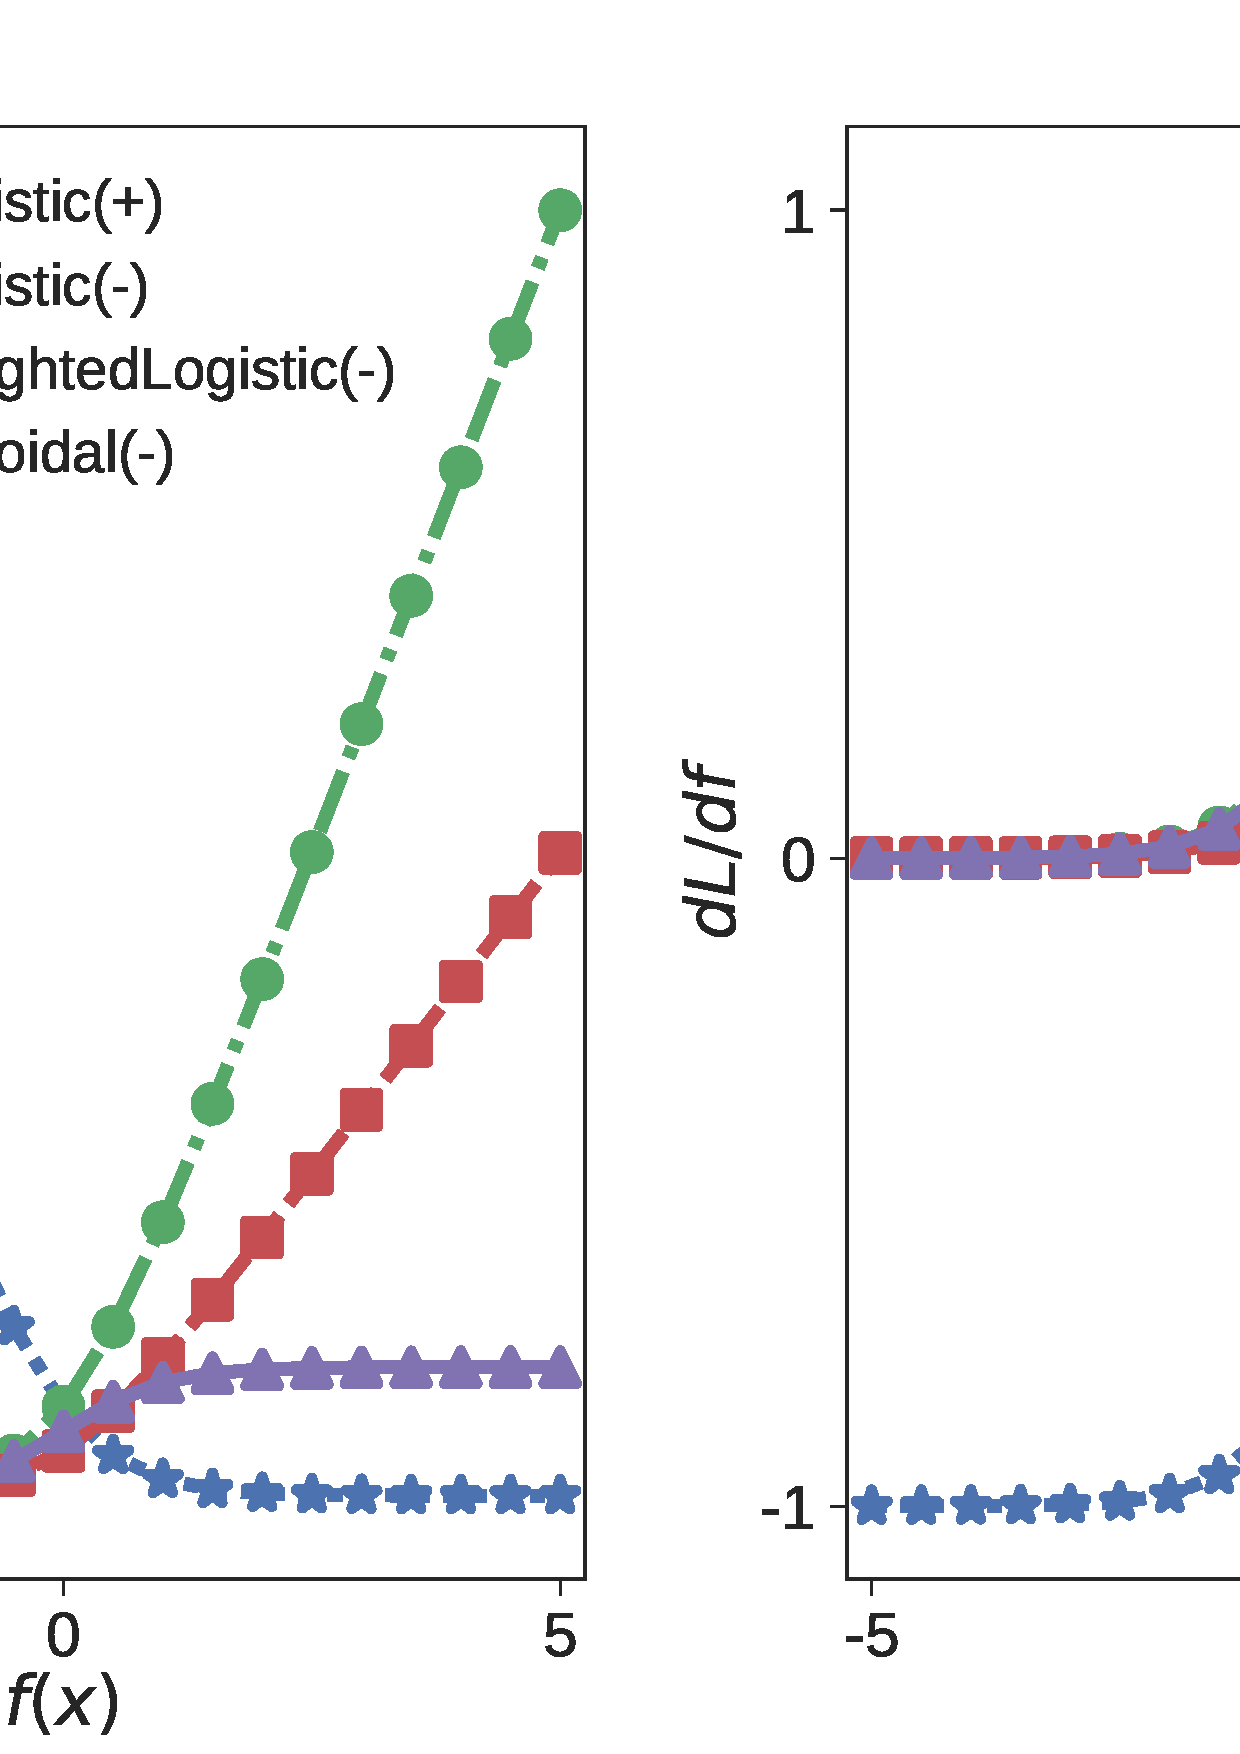
\includegraphics[width=0.95\linewidth]{img/losses.png}
\caption{The Logistic Loss, Weighted Logistic Loss, Exponential Loss and their dirivatives with respect to the model output.}
\label{fig:losses}
\end{figure}


%%%%%%%% FIGURE Varying positive annotating percetage
\begin{figure}[t]
\centering
\fbox{\rule{0pt}{2in} \rule{0.9\linewidth}{0pt}}
  %  \includegraphics[width=0.95\linewidth]{img/}
\caption{Varying percentage of annotated positives 10\%, 20\%, 50\%, 80\% and 100\% with images from CIFAR10 as the positives and images from CIFAR110 as the negatives.}
\label{fig:pct_annotating}
\end{figure}

%%%%%%%% TABLE CIFAR10
\begin{table}[t]
\resizebox{\columnwidth}{!}{
\centering
\begin{tabular}{ll|llll}
Annotation  & Loss & acc. & prec. & rec. & $F_1$ \\
\hline
Complete    & CrossEntropyU.   & $0.87\pm0.01$ & $0.88\pm0.01$ & $0.82\pm0.01$ & $0.85\pm0.01$ \\
50\%(P+N)   & CrossEntropyU.   & $0.83\pm0.01$ & $0.84\pm0.01$ & $0.78\pm0.01$ & $0.80\pm0.01$ \\
50\%P+U     & CrossEntropyU.   & $0.64\pm0.04$ & $0.93\pm0.08$ & $0.34\pm0.02$ & $0.44\pm0.06$ \\
50\%P+U     & WeightedU.       & $0.78\pm0.01$ & $0.75\pm0.01$ & $0.75\pm0.01$ & $0.76\pm0.01$ \\
50\%P+U     & ExponentialU.    & $0.82\pm0.01$ & $0.86\pm0.01$ & $0.73\pm0.01$ & $0.78\pm0.01$ \\
50\%P+U     & BootstrapHard    & $0.74$ & $0.81$ & $0.60$ & $0.67$ \\
50\%P+U     & DropoutReg.      & & & & \\
\end{tabular}
}
\caption{Image classification with positive examples partially annotated. The complete dataset contains images from CIFAR10 as the \textbf{positive} (P) set and images from CIFAR110 as the \textbf{negative} (N) set. The unannotated positive examples from P set construct the \textbf{unlabeled} (U) set together with the N set.}
\end{table}


%%%%%%%% TABLE
\begin{table}[t]
\resizebox{\columnwidth}{!}{
\centering
\begin{tabular}{ll|llll}
Annotation  & Loss & pixel acc. & mean acc. & mean IU & f.w. IU \\
\hline
Complete    & CrossEnt.U    &  &  & & \\
50\%(P+N)   & CrossEnt.U    & & & & \\
50\%P+U     & CrossEnt.U    & & & & \\
50\%P+U     & WeightedU        &  &  & & \\
50\%P+U     & ExponentialU     &  &  & & \\
50\%P+U     & BootstrapHard    &  &  & & \\
50\%P+U     & DropoutReg. & & & & \\
\end{tabular}
}
\caption{Image semantic segmentation with images contain single instance only from the PASCAL VOC2011 segmentation dataset. The complete \textbf{positive} (P) set denotes the foreground instances and the \textbf{negative} (N) set consists of the background. The unannotated instances from P set construct the \textbf{unlabeled} (U) set together with the N set.}
\end{table}


\section{Discussion}
\label{sec:results}

\subsection{Impact of segmentation noises on feature transferability}
\noindent \textit{To summarize the impact of segmentations on feature transferability}
Given the mis-segmentation robustness of feature transferability discussed in section \ref{subsec:robustness}, we proposed to include mis-segmented objects for pre-training.


Pixel independent noise assumption
Logistic loss optimize accuracy, not mean IU


\section{Conclusion}
\label{sec:conclusion}

We studied how to pre-train transferable convolutional weights in the presence of inexhaustive segmentation, misclassification and false segmentation.
Given that including false segmentations of meaningful objects had little impact on the fine-tuning performance of transferred weights, we proposed to include false segmentation objects to learn the pre-trained model.
By contrast, misclassification noises can have negative impacts on feature transferability, but binarizing classes to foreground and background can produce accurate but not necessarily precise labels to train better transferable features.
We presented that for a small pre-training set, binarizing classes can recover the negative influence of misclassification of object segments on the fine-tuning performance of the transferred models.
Inexhaustive segmentation can also negatively affect feature transferability of the pre-trained model.
The decrease of the fine-tuning performance due to the unsegmented objects in the pre-training set can be compensated by modifying the loss function for deep learning models.
We then proposed a class-dependent loss to not over-punish the confident positive predictions for examples with negative labels.
The proposed sigmoidal negative loss was demonstrated to improve both the pre-training and fine-tuning performance of models pre-trained in the presence of inexhaustive segmentations.



{\small
\bibliographystyle{plain}
\bibliography{references}
}

\end{document}
